%%COMPILADO CON XELATEX
\documentclass[12pt,a4paper,roman]{moderncv}



\usepackage{setspace}
%\usepackage[scale=0.75]{geometry}
\usepackage[total={17.5cm,24cm},top=2.0cm, left=1.5cm]{geometry}
%\usepackage{lipsum} % Used for inserting dummy 'Lorem ipsum' text into the template
\moderncvstyle{classic}
\moderncvcolor{burgundy}
\moderncvicons{awesome}
\usepackage{fontspec}
\usepackage{moderntimeline}
\usepackage{datetime}
\newdateformat{monthyeardate}{\monthname[\THEMONTH], \THEYEAR}
\usepackage{tabularx}


\usepackage{ifthen}


\definecolor{color0}{rgb}{0,0,0}% black
\definecolor{color1}{RGB}{30,49,116}% burgundy
\definecolor{color2}{rgb}{0.45,0.45,0.45}% dark grey

\newcommand{\monthnum}{\the\month}
\newcommand{\yearnum}{\the\year}
\newcommand{\MONTH}{%
  \ifcase\the\month
  \or Jan% 1
  \or Feb% 2
  \or Mar% 3
  \or Apr% 4
  \or May% 5
  \or Jun% 6
  \or Jul% 7
  \or Aug% 8
  \or Sep% 9
  \or Oct% 10
  \or Nov% 11
  \or Dec% 12
  \fi}
\makeatletter
\newcommand{\YEAR}{\the\year}
\makeatother





\tlmaxdates{2011}{2022}
\tlwidth{0.8ex}
%\tltext{\small}


%\usepackage{fontawesome}
%\newfontfamily{\FA}{FontAwesome}
%\def\faInstagram{\faicon{instagram}}
%\def\faSkype{\faicon{skype}}
%\def\faLinkedinSquare{\faicon{linkedin-square}}
%\def\faTwitter{\faicon{twitter}}
%\def\faGooglePlusSquare{\faicon{google-plus-square}}
%\def\faFacebookOfficial{\faicon{facebook-official}}
%\def\faCloudDownload{\faicon{cloud-download}}
%\def\faFilePdfO{\faicon{file-pdf-o}}
%\def\faFloppyO{\faicon{floppy-o}}


\definecolor{airbus}{RGB}{8,40,78}

\newcommand{\cventrycustom}[3]{\textcolor{color1}{\scriptsize{\textsc{#1 #2 #3}}}}

\firstname{\Large José Javier \vspace{9pt} \newline} % Your first name
\familyname{\huge \textbf{Rosales Ruiz}} % Your last name
\title{\large \textsc{Aerospace Engineer \newline \textsc{Data Scientist}}}

% All information in this block is optional, comment out any lines you don't need
%\title{ \large Curriculum Vit\ae}


%\date{\today}

\address{ \textcolor{black}{\textsc{PERSONAL DATA}}\\ \\}{}
\mobile{+34 645 526 183}
\mobile{+44 (0)7394 811 610}
%\phone[fixed]{+34 856 216 906}

\email{javier.rosalesruiz@gmail.com }

\extrainfo{\\ \footnotesize \textcolor{black}{\textsc{LAST UPDATE}} \\ \normalsize \today }
%\homepage{www.josejavier-rosalesruiz.com} % The first argument is the url for the clickable link, the second argument is the url displayed in the template - this allows special characters to be displayed such as the tilde in this example
 
%\photo[60pt][0.4pt]{Images/CV_picture} % The first bracket is the picture height, the second is the thickness of the frame around the picture (0pt for no frame)
%\quote{\textsc{Curriculum vit\ae}}

\AfterPreamble{\hypersetup{pdftoolbar=false,        % show Acrobat’s toolbar?
    pdfmenubar=true,        % show Acrobat’s menu?
    pdffitwindow=false,     % window fit to page when opened
    pdfstartview={FitH},    % fits the width of the page to the window
	pdfauthor={José Javier Rosales Ruiz},
    pdftitle={Curriculum Vitae},
    pdfsubject={Aerospace Engineering},
    pdfkeywords={javier.rosalesriz@gmail.com},
    pdfproducer={LaTex},
    pdfcreator={XeLatex}
    pdfnewwindow=true,      % links in new window
    colorlinks=true,       % false: boxed links; true: colored links
    linkcolor=black,          % color of internal links (change box color with linkbordercolor)
    citecolor=black,        % color of links to bibliography
    filecolor=black,      % color of file links
    urlcolor=gray           % color of external links
    }}


\colorlet{secondary}{color1!25!color2}
\usepackage{eurosym}
\usepackage{comment}
\usepackage{scalefnt}
	
\usepackage[margin=10pt,font=small,labelfont=bf]{caption}

%
% TikZ: styles and functions
% 
\usepackage{tikz}
\usetikzlibrary{mindmap,calc,patterns,decorations.pathmorphing,decorations.markings}

\tikzstyle{educationBar} = [rounded corners=1mm,fill=color1, draw=white]
\tikzstyle{educationText} = [rectangle, above=.1cm, align=center, font=\sffamily,scale=1.0]
\tikzstyle{experienceBar} = [rounded corners=1mm,fill=black!40!white, draw=white]
\tikzstyle{experienceText} = [rectangle, below=.1cm, align=center, font=\sffamily,scale=1.00]
	
	
% Function to hide/unhide the grid
% Usage:
% \showTheGrid{1} TRUN ON
% \showTheGrid{0} TRUN OFF
\newcommand{\hreference}{5}
\newcommand{\vreference}{2.5}
\newcommand{\scalefactor}{0.275}
\newcommand{\firstyear}{2011}
\newcommand{\yearspace}{2}

\newcommand{\aspectW}{15}
\newcommand{\aspectH}{3.5}
\newcommand{\showTheGrid}[1]{
    %\draw[step=1cm,gray,very thin, opacity=#1] (0,0) grid (\aspectW,\aspectH);
    \foreach \x in {1,...,\the\numexpr\aspectW} {
    	
		\draw [blue, opacity=#1] (\x,0) -- (\x,0) node[above] {\small{\x}};}
%    \ifodd\x\relax
%		%\draw [blue, opacity=#1] (\x,\aspectH/2) -- (\x,\aspectH/2) node[below] {\huge{\x}};
%		\else
%	\fi }
    \foreach \y in {1,...,\the\numexpr\aspectH} {
		\draw [red, opacity=#1] (0,\y) -- (0,\y) node[left] {\small{\y}};}
%    \ifodd\y\relax
%		%\draw [red, opacity=#1] (\aspectW/2, \y) -- (\aspectW/2, \y) node[right] {\huge{\y}};
%		\else
%	\fi }
		}
		
		
		
% #1 - Type of item
% #2 - \scalefactor*Item number
% #3 - Start of event in years from first year
% #4 - Duration of event in years
% #5 - Title of item
% #6 - MMM/YY of start
% #7 - MMM/YY of end or empty if present.

\newcommand{\timelineitem}[7]{
\draw[thin,black!20!white,->] (2.9,\vreference-\scalefactor*#2) -- (\hreference + #3 -1,\vreference-\scalefactor*#2);
\filldraw[#1] ((\hreference + #3,\vreference -0.1-\scalefactor*#2) rectangle ((\hreference + #4,\vreference + 0.1-\scalefactor*#2);
\node[right] at (0,\vreference-\scalefactor*#2){\tiny{\textsc{#5}}};
%\node[above] at (\hreference + 43/6,\vreference-\scalefactor*0){\tiny{\textsc{Degree in Aerospace Engineering}}};
\node[left] at (\hreference + #3,\vreference-\scalefactor*#2){\tiny{\textsc{#6}}};
\node[right] at (\hreference + #4,\vreference-\scalefactor*#2){\tiny{\textsc{#7}}};
}
	
\includecomment{en} % English language






\begin{document}



\makecvtitle % Print the CV title

%%----------------------------------------------------------------------------------------
%%	WORK EXPERIENCE SECTION
%%----------------------------------------------------------------------------------------
\vspace{-20pt}
\section{\textbf{Experience}}

\cventry{\raisebox{-.15\height}{
\includegraphics[scale=0.07]{Images/Airbus-logo.png}}   \vspace{10mm}
		\raisebox{-.15\height}{\cventrycustom{feb/22}{$\rightarrow$}{Present}} 
			}{\textbf{Business Performance Analyst}}{Airbus}{Broughton}{United Kingdom}{}

\vspace{-25pt}
\cventry{ 	\raisebox{-.15\height}{
\includegraphics[scale=0.07]{Images/Airbus-logo.png}}   \vspace{10mm}
			\raisebox{-.15\height}{\cventrycustom{feb/20}{$\rightarrow$}{feb/22}} 
			}{\textbf{Quality Data \& reporting specialist}}{Airbus}{Broughton}{United Kingdom}{}

\vspace{-25pt}
\cventry{ 	\raisebox{-.15\height}{
\includegraphics[scale=0.175]{Images/Alten-logo.png}}   \vspace{10mm}
			\raisebox{-.15\height}{\cventrycustom{jul/17}{$\rightarrow$}{jan/20}} 
			}{\textbf{Data Scientist \& Software developer}}{Alten}{Puerto Real}{Spain}{}
\vspace{-25pt}
\cventry{ 	\raisebox{-.15\height}{
\includegraphics[scale=0.07]{Images/Airbus-logo.png}}   \vspace{10mm}
			\raisebox{-.15\height}{\cventrycustom{jul/16}{$\rightarrow$}{jul/17}} 
			}{\textbf{Internship at Manufacturing Engineering}}{Airbus}{Puerto Real}{Spain}{}
\vspace{-25pt}
\cventry{ 	\raisebox{-.15\height}{
\includegraphics[scale=0.07]{Images/Airbus-logo.png}} \vspace{10mm} 
			\raisebox{-.15\height}{\cventrycustom{oct/14}{$\rightarrow$}{jan/15}}
			}
			{\textbf{Internship at NC Programs \& Automatization}}{Airbus Defence \& Space}{El Puerto de Santa María}{Spain}{}
%\vspace{3pt}
%\scriptsize{Programming software to organise, upload and normalize data from the automatic machines.}  


%----------------------------------------------------------------------------------------
%	EDUCATION SECTION
%----------------------------------------------------------------------------------------
\vspace{-20pt}
\section{\textbf{Academic background}}
\cventry{\cventrycustom{oct/20}{$\rightarrow$}{Present}}{Master Science in Astronautics and Space Engineering}{Cranfield University}{Cranfield}{}{}
\cventry{\cventrycustom{jan/18}{$\rightarrow$}{mar/21}}{Master Science in Business Analytics and Big Data}{Camilo José Cela University - IMF Business School}{Madrid}{}{}
\cventry{\cventrycustom{sep/16}{$\rightarrow$}{mar/17}}{Master in Professional Development}{Alcalá de Henares University}{Madrid}{}{}
\cventry{\cventrycustom{oct/11}{$\rightarrow$}{apr/18}}{Degree in Aerospace Engineering}{Cádiz University}{Cádiz}{}{Specialising in Airplanes}
%\cventry{2009--2011}{A-level courses}{Compañía de María school}{San Fernando}{Cádiz}{}%{\textit{GPA -- 8.9}}{}  % Arguments not required can be left empty
%\cventry{1996--2009}{Primary and secondary education}{Compañía de María school}{San Fernando}{Cádiz}{}

%\vspace{1\baselineskip}
%\vspace{20pt}
\section{\textbf{Courses}}

%\subsection{\textbf{Language}}

\cventry{\cventrycustom{sep/15}{$\rightarrow$}{jul/16}}{English course for Cambridge Advance certificate}{Bromley College}{London}{}{}
\cventry{\cventrycustom{aug/14}{\&}{aug/15}}{English linguistic immersion}{Menéndez Pelayo International University}{Madrid}{}{}

%\subsection{\textbf{Design}}

\cventry{\cventrycustom{oct/13}{$\rightarrow$}{jun/14}}{CATIA V5R20 (Hybrid Design 2)}{Fundación Universidad Empresa de la provincia de Cádiz (FUECA)}{Cádiz}{}{}%\setlength{\parindent}{4mm}\vspace*{0.0mm}\textcolor{airbus}{\textsc{Hybrid Design 2}}
%\newline{}
%\begin{minipage}[t]{0.5\linewidth}
%\begin{itemize}
%\item Sketcher 
%\item Part design 
%\item Knowledge 
%\item Assembly design
%\end{itemize}
%\end{minipage}%
%\begin{minipage}[t]{0.5\linewidth}
%\begin{itemize}
%\item Generative shape
%\item Generative drafting
%\item Interactive drafting
%\item Wireframe and surface design	
%\end{itemize}
%\end{minipage}
%------------------------------------------------
%}
%\vspace*{3mm}
%\cventry{2013}{Autodesk Inventor Professional}{University of Cádiz (UCA)}{Cádiz}{}{}

%----------------------------------------------------------------------------------------
%	LANGUAGES SECTION
%----------------------------------------------------------------------------------------
%\vspace{1\baselineskip}
\newpage
\section{\textbf{Languages}}

\cvitemwithcomment{\cventrycustom{SPANISH}{}{}}{Native speaker.}{}
\cvitemwithcomment{\cventrycustom{ENGLISH}{}{}}{Proficient.}{}
%\cvitemwithcomment{\cventrycustom{FRENCH}{}{}}{Beginner.}{}

\vspace{1\baselineskip}
\section{\textbf{Professional Timeline}}

%\vspace{1\baselineskip}
%----------------------------------------------------------------------------------------
%	TIMELINE
%----------------------------------------------------------------------------------------

\begin{minipage}{1.0\columnwidth}
  \centering
  
\resizebox{1.0\columnwidth}{!}{ 
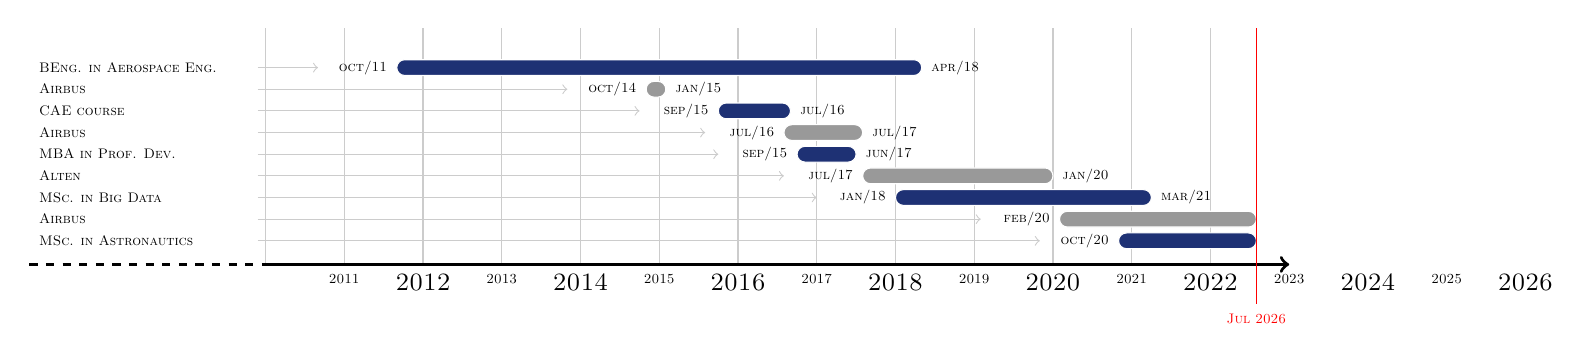
\begin{tikzpicture}






%% The bar with a final arrow
%\shade[rounded corners=0cm, top color=color1!80,bottom color=color1!80] (0,0.7) -- (0,1.3) -- (20.5,1.3) -- (21,1) -- (21,1) -- (20.5,0.70);
%
%% The nodes from 2006 to 2015
%\draw (3,1) node[circle,fill=secondary!30!white,draw]{\small{2011}};
%\draw (5,1) node[circle,fill=secondary!30!white,draw]{\small{2012}};
%\draw (7,1) node[circle,fill=secondary!30!white,draw]{\small{2013}};
%\draw (9,1) node[circle,fill=secondary!30!white,draw]{\small{2014}};
%\draw (11,1) node[circle,fill=secondary!30!white,draw]{\small{2015}};
%\draw (13,1) node[circle,fill=secondary!30!white,draw]{\small{2016}};
%\draw (15,1) node[circle,fill=secondary!30!white,draw]{\small{2017}};
%\draw (17,1) node[circle,fill=secondary!30!white,draw]{\small{2018}};

%\showTheGrid{0}

% Draw vertical lines of grid
\foreach \y in {3,...,\the\numexpr\aspectW} { 
	\draw[black!20!white] (\y,0) -- (\y,\vreference+0.5);}

% Draw x-axis labels of grid (years)
\foreach \x in {2011,...,\yearnum} {
	\ifodd \x \node[below] at (\x-2007,0){\tiny{\textsc{\x}}} 
	\else \node[below] at (\x-2007,0){\small{\textsc{\x}}}\fi;
	
	}

% Education
%
%\node [above right, color1] at (0,9.40){\Large Timeline};

\draw[very thick,->] (3,0) -- (\aspectW+1,0);
\draw[dashed, very thick] (0,0) -- (3,0);



% Create timeline with education and work-experience items using the following args:
% #1 - Type of item
% #2 - \scalefactor*Item number
% #3 - Start of event in years from first year
% #4 - Duration of event in years
% #5 - Title of item
% #6 - MMM/YY of start
% #7 - MMM/YY of end or empty if present.

\timelineitem{educationBar}{0}{-4/12}{76/12}{BEng. in Aerospace Eng.}{oct/11}{apr/18}
\timelineitem{experienceBar}{1}{34/12}{37/12}{Airbus}{oct/14}{jan/15}
\timelineitem{educationBar}{2}{45/12}{56/12}{CAE course}{sep/15}{jul/16}
\timelineitem{experienceBar}{3}{55/12}{67/12}{Airbus}{jul/16}{jul/17}
\timelineitem{educationBar}{4}{57/12}{66/12}{MBA in Prof. Dev.}{sep/15}{jun/17}
\timelineitem{experienceBar}{5}{67/12}{96/12}{Alten}{jul/17}{jan/20}
\timelineitem{educationBar}{6}{72/12}{111/12}{MSc. in Big Data}{jan/18}{mar/21}
\timelineitem{experienceBar}{7}{97/12}{120/12 + \monthnum /12}{Airbus}{feb/20}{}
\timelineitem{educationBar}{8}{106/12}{120/12 + \monthnum /12}{MSc. in Astronautics}{oct/20}{}


\draw[red] (\hreference + 120/12 + \monthnum /12,-0.5) -- (\hreference + 120/12  + \monthnum /12,\vreference+0.5);
\node[below, red] at (\hreference + 120/12  + \monthnum /12 ,-0.5){\tiny{\textsc{\MONTH \ \yearnum }}};

\end{tikzpicture}
}
\end{minipage}
%----------------------------------------------------------------------------------------



%%----------------------------------------------------------------------------------------
%%	COMPUTER SKILLS SECTION
%%----------------------------------------------------------------------------------------
\vspace{1\baselineskip}
\section{\textbf{Skills}}

\begin{center}
\begingroup
\setlength{\tabcolsep}{12pt} % Default value: 6pt
\renewcommand{\arraystretch}{0.65} % Default value: 1
\textcolor{color1}{\textbf{\textsc{Professional}}}\\
\begin{tabular}{l | c | c }
\multicolumn{3}{c}{} \\
\multicolumn{1}{c}{\cventrycustom{TRANSFERABLE}{}{}} & \multicolumn{1}{c}{\cventrycustom{SPECIAL KNOWLEDGES}{}{}} & \cventrycustom{TRAITS}{}{}\\
\tiny{Creating and innovating new methods/tools.} 		& \tiny{Data Science} & \tiny{Responsible}\\
\tiny{Researching and improve processes/tasks.} 		& \tiny{Data Analysis} & \tiny{Reliable}\\
\tiny{Initiating and promoting pioneer ideas.} 			& \tiny{Programming} & \tiny{Persistent}\\
\tiny{Working with numbers and computing.} 				& \tiny{Aerodynamics} & \tiny{Methodical}\\
\tiny{Analyzing data/information and find patterns.} 	& \tiny{Aeroelasticity} & \tiny{Enthusiastic}\\
\tiny{Using my brain to face challenges.} 				& \tiny{Physics} & \tiny{Patient}\\
\tiny{Teaching, training and coaching.} 				& \tiny{Mathematics} & \tiny{Self-motivated}\\
\tiny{Programming \& designing algorithms.} 			& \tiny{Statistics} & \tiny{Dynamic}\\
\tiny{Studying and observing.} 							& \tiny{Machine Learning} & \tiny{Versatile}\\
\tiny{Following through, getting things done.} 			& \tiny{Big Data} & \tiny{Achievement-oriented}     
\end{tabular}
\endgroup
\end{center}


\begingroup
\setlength{\tabcolsep}{12pt} % Default value: 6pt
\renewcommand{\arraystretch}{0.65} % Default value: 1
\begin{center}
\textcolor{color1}{\textbf{\textsc{Computer}}}\\
\begin{tabular}{c  c | c  c | c }
\multicolumn{5}{c}{} \\
\multicolumn{2}{c}{\cventrycustom{CODING}{}{}} & \multicolumn{2}{c}{\cventrycustom{SOFTWARE}{}{}} & \multicolumn{1}{c}{\cventrycustom{OS}{}{}}\\
\tiny{Python \& Pyspark} 			& \tiny{SQL} 		& \tiny{Skywise} 		& \tiny{Spyder/Jupyter} 	& \tiny{Microsoft Windows}  \\
\tiny{JavaScript} 					& \tiny{HTML} 		& \tiny{GSuite} 		& \tiny{RStudio} 			& \tiny{Linux}   \\
\tiny{CSS} 							& \tiny{R} 			& \tiny{MS. Office} 	& \tiny{MySQL} 				& \tiny{Macintosh}  \\
\tiny{VB \& VBS} 					& \tiny{C} 			& \tiny{Tableau}		& \tiny{Pentaho}  			& \tiny{Android OS / iOS}  \\
\tiny{LaTex} 						& \tiny{Batch} 					& \tiny{GitHub} 		& \tiny{Gephi}				& 
\end{tabular}
\end{center}
\endgroup
\vspace{1\baselineskip}
%\cvitem{}{
%\begin{center}
%\begingroup
%\setlength{\tabcolsep}{12pt} % Default value: 6pt
%\renewcommand{\arraystretch}{0.65} % Default value: 1
%\textcolor{color1}{\textbf{\textsc{Professional}}}
%\begin{tabular}{l | c | c }
%\multicolumn{3}{c}{} \\
%\multicolumn{1}{c}{\cventrycustom{FUNCTIONAL}{}{}} & \cventrycustom{SPECIAL KNOWLEDGES}{}{} & \cventrycustom{TRAITS}{}{}\\
%\tiny{Creating and innovating new methods/tools.} 		& \tiny{Data Science} & \tiny{Responsible}\\
%\tiny{Researching and improve processes/tasks.} 		& \tiny{Aerodynamics \& Physics} & \tiny{Reliable}\\
%\tiny{Initiating and promoting pioneer ideas.} 			& \tiny{Data Analysis} & \tiny{Persistent}\\
%\tiny{Working with numbers and computing.} 				& \tiny{Statistics} & \tiny{Methodical}\\
%\tiny{Analyzing data/information and find patterns.} 	& \tiny{Aerodynamics \& Physics} & \tiny{Enthusiastic}\\
%\tiny{Using my brain to face challenges.} 				& \tiny{Aerodynamics \& Physics} & \tiny{Patient}\\
%\tiny{Teaching and training toward new mindsets.} 		& \tiny{Aerodynamics \& Physics} & \tiny{Self-motivated}\\
%\tiny{Programming \& designing algorithms.} 							& \tiny{Aerodynamics \& Physics} & \tiny{Dynamic}\\
%\tiny{Studying and observing.} 							& \tiny{Aerodynamics \& Physics} & \tiny{Versatile}\\
%\tiny{Following through, getting things done.} 							& \tiny{Aerodynamics \& Physics} & \tiny{Achievement-oriented}     
%\end{tabular}
%\endgroup
%\end{center}}
%%\vspace{1\baselineskip}
%
%\cvitem{}{
%\begingroup
%\setlength{\tabcolsep}{12pt} % Default value: 6pt
%\renewcommand{\arraystretch}{0.65} % Default value: 1
%\begin{center}
%\textcolor{color1}{\textbf{\textsc{Computer}}}\\
%\begin{tabular}{c  c | c  c | c }
%\multicolumn{5}{c}{} \\
%\multicolumn{2}{c}{\cventrycustom{CODING}{}{}} & \multicolumn{2}{c}{\cventrycustom{SOFTWARE}{}{}} & \multicolumn{1}{c}{\cventrycustom{OS}{}{}}\\
%\tiny{Python} 		& \tiny{SQL} 	& \tiny{MS Office} 		& \tiny{CATIA V5R20} 	& \tiny{Microsoft Windows}  \\
%\tiny{VB \& VBS} 	& \tiny{R} 		& \tiny{Anaconda} 		& \tiny{Mathematica} 	& \tiny{Android OS}   \\
%\tiny{HTML} 		& \tiny{CSS} 	& \tiny{SQLiteStudio} 	& \tiny{XAMPP} 			& \tiny{Linux}  \\
%\tiny{JavaScript} 	& \tiny{C} 		& \tiny{VirtualBox} 	& \tiny{Eclipse} 		&  \\
%\tiny{LaTex} 		&  				& \tiny{GitHub} 		&  						& 
%\end{tabular}
%\end{center}
%\endgroup
%}


%\subsection{\small{\textbf{Computer}}}
%\cvitem{\cventrycustom{SOFTWARE}{}{}}{Microsoft Office (highly proficient), Anaconda (Jupyter, Spyder and RStudio), SQLiteStudio, VirtualBox, GitHub, CATIA V5R20, Eclipse, XAMPP, AutoCAD, Mathematica, MatLab and Ansys Fluent.}
%\cvitem{\cventrycustom{PROGRAMMING}{}{}}{VBS  \& VBA (highly proficient), Python, R, SQL, JavaScript, HTML, CSS, \textsc{C}, SAP Scripting and LaTex.}
%\cvitem{\cventrycustom{OS}{}{}}{Linux and Microsoft Windows.}
%\vspace{1\baselineskip}
%\subsection{\small{\textbf{Personal}}}

%\cvitem{\cventrycustom{CAPACITY}{}{}}{Effective and structured personal organisation with ability to remain composed and focused under pressure.}
%\cvitem{\cventrycustom{VERSATILITY}{}{}}{Ability to reach succesfully the expertise to work on new projects learning new methods.}
%\cvitem{\cventrycustom{INITIATIVE}{}{}}{Self motivated with the ability and enthusiasm to find creative solutions. Actively pursuing to improve and develop new skills.}
%\cvitem{\cventrycustom{COMMUNICATION}{}{}}{Strong verbal and written communication skills.}



%----------------------------------------------------------------------------------------
%	INTERESTS SECTION
%----------------------------------------------------------------------------------------
%\vspace{1\baselineskip}
\section{\textbf{Interests}}

\renewcommand{\listitemsymbol}{-~} % Changes the symbol used for lists

\cvlistdoubleitem{Data Science}{Data Analysis}
\cvlistdoubleitem{Machine learning}{Big Data}
\cvlistdoubleitem{Statistics}{Mathematics}
\cvlistdoubleitem{Physics}{Aerodynamics}
\cvlistdoubleitem{Astrodynamics}{Space Engineering}




\end{document}